\documentclass{article}

% General physics constructs
\newcommand{\bra}[1]{\langle #1 |}
\newcommand{\ket}[1]{| #1 \rangle }
\newcommand{\braket}[2]{\langle #1|#2\rangle}
\newcommand{\bbraket}[3]{ \langle #1 | #2 | #3 \rangle }
\newcommand{\norm}[1]{\| #1\|}
\newcommand{\avg}[1]{\left \langle #1 \right \rangle}
\newcommand{\angavg}[1]{\left \langle #1 \right \rangle}
\newcommand{\abs}[1]{\left \lvert #1 \right \rvert}
\newcommand{\VS}{\textit{\textbf{V}}}
\newcommand{\Tr}{\textrm{Tr}}
\renewcommand{\Re}{\textrm{Re}}
\renewcommand{\Im}{\textrm{Im}}
\newcommand{\basis}[1]{\{\ket{#1}\}}

\newcommand{\omegaqubit}{\omega_{10}}

% Figures. Example usage:
% \quickfig{\columnwidth}{my_image}{This is the caption}{fig:my_fig}
\DeclareRobustCommand{\quickfig}[4]{
\begin{figure}
\begin{centering}
\includegraphics[width=#1]{#2}
\par\end{centering}
\caption{#3}
\label{#4}
\end{figure}
}

\DeclareRobustCommand{\quickwidefig}[4]{
\begin{figure*}[h]
\begin{centering}
\includegraphics[width=#1]{#2}
\par\end{centering}
\caption{#3}
\label{#4}
\end{figure*}
}

%Packages
\usepackage{amsmath}
\usepackage{amstext}
\usepackage{amssymb}
\usepackage{appendix}
\usepackage{coseoul}
\usepackage{enumerate}
\usepackage{graphicx}
\usepackage{import}
\usepackage{lscape}
\usepackage{modular}

\usepackage[pdfpagemode=UseNone,pdfstartview=FitH,colorlinks=true,linkcolor=blue,citecolor=blue,urlcolor=blue]{hyperref}
\usepackage[all]{hypcap}


\newcommand{\citeinternaltype}{Ref.\,}
\newcommand{\Citeinternaltype}{Reference}
\newcommand{\citeinternalref}[1]{\cite{Sank:#1}}


\title{Quantum Harmonic Oscillator}
\author{Daniel Sank}
%\author{Daniel Sank \\ \small{Google Quantum AI \\ Formerly Department of Physics, UCSB}}

\date{16, October 2008}

\begin{document}

\maketitle

Here I collect useful formulae regarding the quantum simple harmonic oscillator.
The idea is to provide expressions for things like matrix elements and zero point fluctuations in terms of generalized Hamiltonian parameters so that they can easily be applied to any harmonic system.

\section{General Form}

The general form of the Hamiltonian for a harmonic oscillator is \begin{equation}
H = \frac{1}{2} \alpha u^2 + \frac{1}{2} \beta v^2 \qquad [u,v]= i \gamma . \end{equation}
Using dimensionless operators \begin{align}
X \equiv \frac{1}{\sqrt{2 \gamma}} \left( \frac{\alpha}{\beta}\right)^{1/4}\,u &\quad \textrm{and} \quad Y \equiv \frac{1}{\sqrt{2 \gamma}} \left( \frac{\beta}{\alpha} \right)^{1/4}\,v \\
[X,Y] &= i/2 \end{align}
we get a new form of the Hamiltonian \begin{equation}
H = \gamma \sqrt{\alpha \beta} \left[ X^{2} + Y^{2} \right] .
\end{equation}
We also introduce raising and lowering operators $a$ and $a^{\dagger}$ defined by the following equations \begin{align}
a = X+iY &\qquad a^{\dagger} = X-iY \nonumber \\
X = \frac{1}{2}\left(a+a^{\dagger}\right) &\qquad Y = \frac{-i}{2}\left(a-a^{\dagger}\right) \\
[ a, a^{\dagger} ] &= 1 . \end{align}
Writing down the expression for $a^{\dagger}a$ and expanding it in terms of the $X$ and $Y$ operators, we find \begin{align*}
\gamma \sqrt{\alpha \beta} ( a^{\dagger} a ) & = \gamma\sqrt{\alpha\beta} (X-iY)(X+iY)\\
 & = \gamma\sqrt{\alpha\beta} \left(X^2 + iXY - iYX + Y^2 \right)\\
 & = \gamma\sqrt{\alpha\beta} \left(X^2 + Y^{2} + i \left[ X,Y \right] \right)\\
 & = \gamma\sqrt{\alpha\beta} \left(X^2 + Y^{2} - 1/2 \right)\\
 & = H - \frac{1}{2}\gamma\sqrt{\alpha\beta} \\
\textrm{so}\qquad H & = \left( a^{\dagger}a + \frac{1}{2} \right) \gamma\sqrt{\alpha\beta}. \end{align*}
It will be shown below from Heisenberg's equations of motion that \begin{equation}
\hbar\omega=\gamma\sqrt{\alpha\beta} \end{equation}
which means that the Hamiltonian can be written as \begin{equation}
H=\hbar\omega\left(a^{\dagger}a+\frac{1}{2}\right). \end{equation}

\subsection{Zero point fluctuation}

The zero point fluctuation of $X$ is \begin{equation}
\bbraket{0}{X^2}{0} = \frac{1}{4}\bbraket{0}{a^2 + aa^{\dagger} + a^{\dagger}a + a^{\dagger^2}}{0} = 1/4 \end{equation}\
which we write compactly as \begin{equation}
\langle X^2 \rangle_0 = \langle Y^2 \rangle_0 = 1/4 . \end{equation}
From this, we compute the zero point fluctuations of $u$ and $v$, \begin{equation}
\langle u^2 \rangle_0 = \frac{1}{2}\gamma \sqrt{\beta / \alpha} \quad \langle v^2 \rangle_0 = \frac{1}{2}\gamma \sqrt{\alpha / \beta} . \end{equation}
Defining $u_{\textrm{zpf}}^2 \equiv \langle u^2 \rangle_0 $ we have \begin{equation}
X = \frac{1}{2}\frac{u}{u_{\textrm{zpf}}} \quad Y = \frac{1}{2}\frac{v}{v_{\textrm{zpf}}} \end{equation}

\section{Algebra}

From the commutator $ [a,a^{\dagger}]=1 $ and the conjugate variables formulae in \citeinternaltype \citeinternalref{quantumMechanics} it follows that \begin{equation}
[a,T] = \frac{\partial T}{\partial a^{\dagger}} \qquad [a^{\dagger},T] = -\frac{\partial T}{\partial a}\end{equation}
as long as $T$ is written in normal order form (all $a^{\dagger}$ operators to the left of all $a$ operators).
This is extremely useful when computing dynamics in the Heisenberg or interaction picture, as will be shown in the next section.

\section{Equations of Motion}

The Heisenberg equation of motion for the $a$ operator is \begin{eqnarray*}
i\hbar d_{t}a & = & [a,H] \\
& = & \gamma\sqrt{\alpha\beta}[a,a^{\dagger}a+\frac{1}{2}] \\
& = & \gamma\sqrt{\alpha\beta}\frac{\partial(aa^{\dagger})}{\partial a^{\dagger}} \\
& = & \gamma\sqrt{\alpha\beta}\,a \end{eqnarray*}
giving \begin{equation}
\dot{a} = -i\frac{\gamma\sqrt{\alpha\beta}}{\hbar}a .\end{equation}
Solving this simple differential equation yields \begin{equation}
a(t) = a(0)\exp\left[-i \omega t \right] \quad \textrm{and} \quad a^{\dagger}(t) = a^{\dagger}(0)\exp\left[i \omega t \right] . \end{equation}
where $\omega \equiv \gamma\sqrt{\alpha\beta}/\hbar$ as claimed above.
Note that the evolution of $a$ in the phase plane is $\emph{clockwise}$, ie. the phasor convention we inherit from Schrodinger's (Heisenberg's) equation has a $-i$.
This is important interpreting the meaning of positive and negative energy in a quantum calculation.


\section{Coherent States}

Suppose we want to find an eigenvector of the lowering operator.
For starters we know that the state $\ket{0}$ is an eigenket of the lowering operator with eigenvalue $0$.
We also know that to translate $a$ by an amount $\phi$ we should apply the operator $\exp[\phi a^{\dagger}]$.
Therefore we guess that the general eigenket of $a$ is
\begin{equation*}
  \ket{\phi}_?
  = e^{\phi a^{\dagger}}\ket{0}
  = \sum_{n=0}^\infty \frac{\phi^n (a^\dagger)^n}{n!} \ket{0}
  \, .
\end{equation*}
With this definition we have
\begin{align*}
  a \ket{\phi}_?
  &= a e^{\phi a^\dagger} \ket{0} \\
  &= \sum_{n=1}^\infty \frac{\phi^{n}}{n!} a (a^{\dagger})^{n} \, \ket{0}
\end{align*}
where the $n=0$ term vanishes because $a\ket{0} = 0$.
As $[a,(a^{\dagger})^{n}] = \partial_{a^\dagger}(a^\dagger)^n = n(a^{\dagger})^{n-1}$ we have
\begin{equation}
  a(a^{\dagger})^{n}=(a^{\dagger})^{n}a+n(a^{\dagger})^{n-1}
\end{equation}
so then
\begin{equation}
  a\ket{\phi}_? = \sum_{n=1}^{\infty}\frac{\phi^{n}}{n!} \left((a^{\dagger})^{n}a+n(a^{\dagger})^{n-1} \right) \, \ket{0}
\end{equation}
and since $a\ket{0}=0$ we can drop the $(a^{\dagger})^{n}a$ term, leaving,
\begin{align*}
  a\ket{\phi}_?
  &= \sum_{n=1}^{\infty}\frac{\phi^{n}}{n!} \left(n(a^{\dagger})^{n-1} \right) \, \ket{0} \\
  &= \phi \, \sum_{n=1}^\infty \frac{\phi^{n-1}}{(n-1)!}(a^{\dagger})^{n-1} \, \ket{0} \\
  &= \phi \, \sum_{n=0}^\infty \frac{\phi^n}{n!}(a^{\dagger})^n \, \ket{0} \\
  &= \phi\ket{\phi}_?
\end{align*}
so the kets $\ket{\phi}_?$ are eigenkets of $a$ as we hoped.
However, they aren't propertly  normalized,
\begin{align*}
  _?\braket{\phi}{\phi}_?
  &= \sum_{m,n=0}^\infty \bra{0} a^m \frac{\phi^{*^m}}{m!} \frac{\phi^n}{n!}(a^\dagger)^n \ket{0} \\
  &= \sum_{n=0}^\infty \frac{\lvert \phi \rvert^{2n}}{n!} \\
  &= e^{\lvert \phi \rvert^2}
\end{align*}
so the properly normalized states called ``coherent states'' are
\begin{equation}
  \boxed{
    \ket{\phi} = e^{-\frac{1}{2} \lvert \phi \vert^2 } e^{\phi a^\dagger} \ket{0}
  }
  \, .
\end{equation}
Another way to write the coherent state is
\begin{equation*}
  \ket{\phi} = e^{-\frac{1}{2} \abs{\phi}^2} e^{\phi a^\dagger} e^{-\phi^* a} \ket{0}
\end{equation*}
which works because $\exp \left( -\phi a \right) \ket{0} = \ket{0}$.
Using the BCH theorem we find
\begin{equation*}
  e^{-\frac{1}{2} \abs{\phi}^2} e^{\phi a^\dagger} e^{-\phi^* a}
  = e^{\phi a^\dagger - \phi^* a}
\end{equation*}
so
\begin{equation}
  \boxed{
    \ket{\phi} = \underbrace{\exp \left( \phi a^\dagger - \phi^* a \right)}_{D(\phi)} \ket{0}
  }
\end{equation}
where $D(\phi)$ is called the ``displacement operator''.
The displacement operator is convenient for mathematical manipulations.
For example, the derivative of a coherent state with respect to its eigenvalue
\begin{align*}
  \partial_{\phi}\ket{\phi}
  &= \frac{\partial}{\partial \phi} \sum_{n=0}^\infty \frac{\phi^n (a^\dagger)^n}{n!} \ket{0} \\
  &= \sum_{n=1}^{\infty}\frac{\phi^{n-1}}{(n-1)!}a^{\dagger}(a^{\dagger})^{n-1} \, \ket{0} \\
  &= a^{\dagger}\ket{\phi}
\end{align*}
can be remembered easily as
\begin{align}
  \partial_\phi \ket{\phi}
  &= \partial_\phi D(\phi) \ket{0} \nonumber \\
  &= \partial_\phi \exp \left(\phi a^\dagger - \phi^* a \right) \nonumber \\
  &= a^\dagger \exp \left(\phi a^\dagger - \phi^* a \right) \nonumber \\
  &= a^\dagger \ket{\phi} \, .
\end{align}


A very important identity that is used in the context of Wigner functions
is the completeness relation
\begin{equation}
  \int \frac{d\Re(\phi)d\Im(\phi)}{\pi} e^{-\phi^{*}\phi}\ket{\phi}\bra{\phi}
  = \mathbb{I}
\end{equation}


\levelstay{Driving} \label{sec:driving}

\leveldown{Capacitive driving}

We next consider driving signals applied to the circuit.
We attach a driving voltage source to our parallel LC through a capacitor $C_d$, as shown by the dotted elements in Fig.\,\ref{Fig:singleCircuit}.
The capacitor $C_d$ is required to prevent the driving circuit from completely ruining the coherence of the main circuit.
Without the capacitor, the loaded quality factor $Q_d$ of the main circuit due to the drive circuit would be \citeinternalref{loadedMode}
\begin{equation}
Q_d = R_d / Z_{LC} .
\end{equation}
With typical circuit impedances in the range 10's to 100's of Ohms, and RF source resistances of $50\,\Omega$\,\footnote{Commercial RF devices essentially \emph{all} use 50 \, $\Omega$ output impedance. This is simply due to the fact that a coaxial transmission line of reasonable size has near $50 \, \Omega$ impedance. The impedance depends logarithmically on geometric parameters and so cannot be significantly varied. 50$ \, \Omega$ has been chosen as a common standard.}, we have $Q_d \approx 1$ which is far too low to be useful in a quantum device.\footnote{The energy relaxation time of the circuit is $T_1 = Q_d / \omega$, so for a 1 GHz device $Q_l=1$ corresponds to $T_1=0.16 \, \text{ns}$.}

The coupling capacitor $C_d$ helps preserve the circuit coherence.
If $C_d$ is sufficiently small, its impedance $Z_{C_d} = 1/i\omega C_d$ is large and the current flowing through $R_d$ is reduced.
Therefore, $C_d$ prevents the process by which energy from the oscillator gets into $R_d$ and is lost.
To be specific, in the limit $Z_{C_d} \gg R_d$ the loaded quality factor of the oscillator is \citeinternalref{loadedMode}
\begin{equation}
Q_l = \left( \frac{C}{C_d} \right)^2 \frac{Z_{LC}}{R_d} .
\end{equation}
Therefore, a small $C_d$ preserves the circuit's coherence.
However, decoupling the drive line from the driving voltage source with a small $C_d$ also limits the speed with which we can control the circuit, so a balance must be struck.
This balance is discussed in full quantitative detail later.

Let's now turn back to formal analysis of the driven circuit, starting with a qualitative prediction.
The main capacitor $C$ is shunted by the series combination of the coupling capacitor $C_d$, and the resistor $R_d$.
Because  $Z_{C_d} \gg R_d$ the impedance of the driving circuit is dominated by $C_d$ which simply adds in parallel with $C$.
Therefore, we expect the effective capacitance of the mode to be $C+C_d$.

Denoting the time dependent driving voltage by $V_d(t)$ and ignoring for now the resistance of the source, we work out Kirchhoff's equation of motion for the driven system, resulting in
\begin{equation}
\frac{1}{1+C/C_d} \dot{V}_d = \ddot{\Phi} + \frac{\omega_0^2}{1 + C_d/C} \Phi. \end{equation}
This is totally sensible: the drive strength increases as $C_d$ increases, and the resonance frequency of the LC mode has shifted due to the new capacitance.
This equation of motion is produced by the Lagrangian
\begin{equation}
\mathcal{L} = \frac{1}{2}C \dot{\Phi}^2 - \frac{1}{2L}\Phi^2 + \frac{1}{2} C_d \left( \dot{\Phi} - V_d \right)^2 \, .
\end{equation}
For the sake of identifying canonical coordinates we consider the case $V_d=0$, resulting in canonical variables
\begin{equation*}
  \Phi
  \qquad \textrm{and} \qquad
  \frac{\partial \mathcal{L}}{\partial \dot{\Phi}} = \left( C + C_d \right) \dot{\Phi} \equiv Q
\end{equation*}
just as before, except that now the capacitance associated to the momentum $Q$ is $C+C_d$ instead of just $C$, which makes sense because $C_d$ is in parallel with $C$.
The Hamiltonian is
\begin{equation}
  H = \frac{Q^2}{2 (C + C_d)} + \frac{\Phi^2}{2L} \, .
\end{equation}
Now we consider what happens when the drive turns on.
The term added to the Lagrangian by the drive is
\begin{equation}
  \mathcal{L}_d = \frac{1}{2}C_d V_d(t)^2 - C_d \dot{\Phi} V_d(t) \, .
\end{equation}
The first term is of no consequence as it does not involve the dynamical variables.
The second term couples the drive to the momentum $Q$, resulting in a Hamiltonian term
\begin{equation*}
H_d
  = C_d \dot{\Phi}V_d(t)
  = \frac{1}{1+C/C_d} Q V_d(t) \, . \label{eq:sec:driving:H_dVsCircuitParams}
\end{equation*}
Now suppose the drive is on resonance with one particular transition $\ket{n} \rightarrow \ket{n+1}$ and far off resonance from any other transition.
In this case we can restrict the analysis to just the states involved in the driven transition.\footnote{The restriction to two levels whose transition is on resonance with the drive is properly justified in the rotating frame, discussed later.}
Because the wave functions of a one-dimensional quantum Hamiltonian are real and because $Q = -i \hbar d/d\Phi$, we can write
\begin{equation*}
  \bbraket{n}{Q}{n+1} = -i \abs{\bbraket{n}{Q}{n+1}} \, ,
\end{equation*}
and using that we can write $H_d$ as
\begin{align*}
  H_d
  &= \frac{V_d(t)}{1 + C / C_d}
    \left[ \begin{array}{cc}
      \bbraket{n}{Q}{n} & \bbraket{n}{Q}{n+1} \\
      \bbraket{n+1}{Q}{n} & \bbraket{n+1}{Q}{n+1}
    \end{array}\right] \\
  &= \frac{V_d(t)}{1 + C / C_d} \left(
      \frac{S_Q}{2} \mathbb{I}
    + \frac{\Delta_Q}{2} \sigma_z
    + \abs{\bbraket{n}{Q}{n+1}} \sigma_y
  \right)
\end{align*}
where $S_Q \equiv \bbraket{n}{Q}{n} + \bbraket{n+1}{Q}{n+1}$ and $\Delta_Q \equiv \bbraket{n}{Q}{n} - \bbraket{n+1}{Q}{n+1}$.
Going back to our definition of the $a$ operator, we can rewrite $Q$ as
\begin{equation*}
  Q = -i Q_\text{zpf} (a - a^\dagger)
\end{equation*}
and if the system is approximately harmonic, then $\bbraket{n}{Q}{n} \approx 0$, $\bbraket{n+1}{Q}{n+1} \approx 0$, and $\bbraket{n}{Q}{n+1} \approx Q_\text{zpf} \sqrt{n+1}$, so
\begin{equation*}
  H_d = \frac{V_d(t)}{1 + C / C_d} \sqrt{n+1} \, Q_\text{zpf} \, \sigma_y
  \, .
\end{equation*}
Later, we will express this driving Hamiltonian in the rotating frame of the qubit.
However, we can already see one important point: the coupling of the drive signal to the circuit scales with the zero point fluctuations in the circuit's charge, and therefore inversely with $\sqrt{Z_{LC}}$.
In other words, low impedance would appear to give stronger coupling.
However, one must be careful about what is being held constant.
Assuming fixed $\omega_{LC}$ and $C \gg C_d$, we find that the drive Hamiltonian is proportional to
\begin{equation}
  \omega_{LC} \sqrt{Z_{LC}}
\end{equation}
which increases for \emph{increasing} impedance.
These same arguments apply to qubit-qubit coupling, as will be described below.

\textbf{Summary - Simple derivation:} The energy stored in the drive capacitor is $E_d = \frac{1}{2}C_d\left( V_d - V_q \right)^2$.
Keeping only the terms involving both the qubit and drive voltages yields \begin{equation}
E_d = - C_d V_d V_q = - C_d V_d \frac{Q}{C} \end{equation}
where $Q$ is the qubit charge.
This matches the full result up to the sign, in the practical limit $C \gg C_d$.


\levelstay{Inductive driving}

\begin{figure}
\begin{centering}
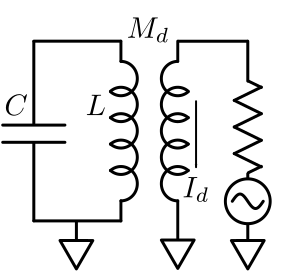
\includegraphics[width=5cm]{inductive_drive.pdf}
\par\end{centering}
  \caption{Parallel LC driving through a mutual inductance.}
\label{fig:qubits.inductive_drive}
\end{figure}

We now consider the case in which we drive by applying current into an inductor which is coupled to the qubit inductor through a mutual inductance $M_d$, as shown in Figure \ref{fig:qubits.inductive_drive}.
With a drive current $I_d(t)$ Kirchhoff's law for the circuit yields the equation of motion
\begin{equation}
  \ddot{\Phi} + \omega_{LC}^2 \Phi = I_d \, \omega_{LC}^2 M_d \, .
\end{equation}
This equation is reproduced by the Lagrangian
\begin{equation}
  \mathcal{L} = \frac{1}{2}C \dot{\Phi}^2 - \frac{1}{2L} \Phi^2 + \frac{M_d}{L}I_d(t) \Phi \, .
\end{equation}
The momentum conjugate to $\Phi$ is
\begin{equation}
  \frac{\partial \mathcal{L}}{\partial \dot{\Phi}} = C \dot{\Phi} = Q
\end{equation}
and the Hamiltonian is
\begin{equation}
  H
  = Q \dot{\Phi} - \mathcal{L}
  = \frac{Q^2}{2C} + \frac{\Phi^2}{2L} - \frac{M_d}{L} I_d(t) \Phi
\end{equation}
so the driving Hamiltonian is
\begin{equation}
  H_d = - \frac{M_d}{L}I_d(t) \Phi \, .
\end{equation}
Note that adding a parallel junction to the circuit does \emph{not} change the form of $H_d$; the junction adds a term $(I_c \Phi_0 / 2\pi)\cos(\pi \Phi / \Phi_0)$ to the Lagrangian, but this term does not couple to $I_d$.
Just as we did for the capacitive drive, we can express the restriction of the inductive drive Hamiltonian two a two-level subspace as
\begin{equation*}
  H_d = -\frac{M_d}{L} I_d(t) \left(
      \frac{S_\Phi}{2} \mathbb{I}
    + \frac{\Delta_\Phi}{2} \sigma_z
    + \abs{\bbraket{n}{\Phi}{n+1}} \sigma_x
  \right)
\end{equation*}
where $S_\Phi = \bbraket{n}{\Phi}{n} + \bbraket{n+1}{\Phi}{n+1}$ and $\Delta_\Phi = \bbraket{n}{\Phi}{n} - \bbraket{n+1}{\Phi}{n+1}$.
Just as in the capacitive case, we can rewrite $\Phi$ in terms of the raising and lowering operators
\begin{equation*}
  \Phi = \Phi_\text{zpf} (a + a^\dagger)
\end{equation*}
and if the system is approximately harmonic then
\begin{equation*}
  H_d = - \frac{M_d}{L} I_d(t) \sqrt{n+1} \, \Phi_\text{zpf} \, \sigma_x
  \, .
\end{equation*}


\bibliographystyle{plain}
\bibliography{../../Bibliography/references_main,../../Bibliography/references_local}

\end{document}
